\documentclass[11pt]{article}
\usepackage[a4paper,margin=0.92in]{geometry}
\usepackage{amsmath,amssymb,amsthm,mathtools}
\usepackage{booktabs,array}
\usepackage{graphicx}
\usepackage{xcolor}
\usepackage[hidelinks]{hyperref}
\hypersetup{
  pdftitle={Architecture-Dependent Decoherence Suppression in Passive Quantum Networks},
  pdfauthor={Lluis Eriksson},
  pdfsubject={Irreducible channel mixing, passive quantum networks, decoherence rates, and dwell-time cost}
}
\usepackage[nameinlink,capitalise]{cleveref}
\usepackage{microtype}

\newtheorem{theorem}{Theorem}[section]
\newtheorem{proposition}[theorem]{Proposition}
\newtheorem{lemma}[theorem]{Lemma}
\newtheorem{corollary}[theorem]{Corollary}
\theoremstyle{definition}
\newtheorem{definition}[theorem]{Definition}
\theoremstyle{remark}
\newtheorem{remark}[theorem]{Remark}
\newtheorem{limitation}[theorem]{Limitation}

\newcommand{\C}{\mathbb{C}}
\newcommand{\T}{\mathbb{T}}
\newcommand{\cR}{\mathcal{R}}
\newcommand{\cI}{\mathcal{I}}
\newcommand{\diag}{\operatorname{diag}}
\newcommand{\Span}{\operatorname{span}}
\newcommand{\op}{\mathrm{op}}
\newcommand{\dd}{\mathrm{d}}
\newcommand{\e}{\mathrm{e}}

\title{Architecture-Dependent Decoherence Suppression in Passive Quantum Networks:\\
Irreducible Channel Mixing, Squared Rate Gaps, and the Price in Dwell Time}
\author{Lluis Eriksson}
\date{10 August 2026}

\begin{document}
\maketitle

\begin{abstract}
Can passive reservoir filtering suppress decoherence more strongly when its
channel mixing is irreducible, even after passband responses and rational
complexity are fixed?  We give an explicit affirmative separation, together
with the resource that pays for it.  For every integer $S\geq5$ we construct a
causal three-signal/three-loss-port inner transfer whose signal block $G_S$ is
a rational Schur function with numerator degree at most $S+4$ and common
denominator degree $S$.  It obeys $3(S-1)$ exact delayed tangential
calibrations in a pass arc; every three calibration signatures span $\C^3$.
On two stop arcs,
\[
\sup\|G_S\|_{\op}\leq
 \varepsilon_S:=\left(\frac{\pi S}{6}+\frac12\right)\e^{-9S/20}.
\]
In contrast, every transfer of the same bidegree that has a constant
nontrivial reducing channel and obeys the same calibrations has stopband norm
at least one.  The proof is a scalar root-count obstruction exposed by the
full-spark signatures.  We strengthen this discontinuous-looking statement:
for calibration defect $\delta$ and sampled reducing-line defect $\beta$, the
comparator leakage is at least $[1-C_S(\delta+\beta)]_+$, where $C_S$ is an
explicit finite-matrix constant.  A scalar Schur construction then proves
that every valid $C_S$ must grow at least as $2\e^{9S/20}(1+o(1))$; uniform
robustness is impossible for these calibrations.  The lossless completion uses only three scalar
Blaschke all-pass elements, balanced interferometers and paraunitary delays,
so physical passivity is verified directly rather than inferred from an
unconstrained interpolation.  For a bath spectral density
$j_-I\preceq J\preceq j_+I$, the filtered Kossakowski matrix therefore has
norm at most $j_+\varepsilon_S^2$, whereas every reducing comparator retains a
directional rate at least $j_-$.  In a closed Markov pure-dephasing model the
three auxiliary vacuum ports contribute exactly the architecture-independent
baseline $\kappa_0I$; hence the observable total-rate advantage is at least
$(\kappa_0+j_-)/(\kappa_0+j_+\varepsilon_S^2)$ and saturates at the vacuum
floor.  The separation is not free: if a finite Blaschke product of
degree $S$ yields signal leakage at most $\varepsilon<1$ on an arc of length
$L$, its peak group delay is at least
$LS/(16\arcsin\varepsilon)$.  Our family has exponentially large delay.  Thus
under a peak-delay budget $D$, the rate-improvement factor is at most
$\csc^2(LS/(16D))$, asymptotically quadratic in $D/S$.  Irreducible passive
mixing can therefore move a coherence-maintenance boundary, but it
moves the required resource into long-lived passive memory rather than
erasing it.  Exact arithmetic, dense-grid unitarity audits and all figures are
reproduced by the linked public source package.
\end{abstract}

\section{Question, result, and non-claims}

Quantum filter functions translate control protocols into frequency-resolved
noise response \cite{PazSilvaViola2014,CerfontaineEtAl2021}, and passive linear
quantum systems admit network and realization theories that preserve the
canonical commutation relations \cite{GoughJames2009,GoughGohmYanagisawa2009,GoughZhang2015}.
Tangential interpolation can itself be made physical-realizability- and
passivity-preserving \cite{TechakesariNurdin2017}.  Blaschke--Potapov factors
have also been used to identify trapped modes in delayed passive quantum
networks \cite{TabakMabuchi2016}.  None of those ingredients is claimed as new.

The narrower question here is architectural.  Suppose that a multichannel
filter must match many directional responses exactly, has a fixed rational
bidegree, and remains passive.  Is a device whose channels split after one
frequency-independent rotation necessarily as capable as one whose channel
geometry changes with frequency?  The answer is no.  We prove an exponential
signal-level gap between an explicit irreducible signal block and every
constant-channel reducing comparator.  Passing that gap through a uniformly
nondegenerate bath spectral density squares the suppression exponent.  We
then prove a delay lower bound that prevents the architecture theorem from
being misread as a free thermodynamic advantage.

This result develops the resource-boundary viewpoint of
\cite{ErikssonCut2026} in a direction orthogonal to spatial buffer thickness.
The protected object is a frequency-resolved coupling channel.  The filter can
move the rate boundary by changing its channel architecture, but poles near
the unit circle store the resource as dwell time.  The paper makes no claim to
derive the Born rule, select outcomes, solve an interacting many-body buffer,
or show that a small thermodynamic lower bound is achievable.

The contributions are:
\begin{enumerate}
  \item an explicit six-port causal inner completion, with no appeal to a
  black-box synthesis theorem;
  \item a fixed-bidegree irreducible/reducible separation under exact
  full-spark tangential calibrations;
  \item an approximate-calibration theorem with a computable conditioning
  constant, and a matching exponential obstruction to uniform robustness;
  \item a squared separation for filtered Kossakowski matrices and a closed
  Ramsey model in which all vacuum ports are accounted for;
  \item a general delay-price theorem for the scalar all-pass mechanism;
  \item an exact no-go showing why the earlier real-symmetric quadratic
  certificate cannot be made globally passive by scalar rescaling; and
  \item a reproducible ledger linking every numerical statement to code
  \cite{ErikssonRepository2026}.
\end{enumerate}

\section{Passive transfer model and comparison class}

We use the unit-disc convention.  A matrix transfer $\mathsf{S}(z)$ is
\emph{inner} when it is analytic for $|z|<1$ and unitary almost everywhere on
$\T=\{z:|z|=1\}$.  A principal block $G(z)$ of an inner transfer is Schur:
$\|G(z)\|_{\op}\leq1$ in the disc and on its regular boundary points.  In a
passive quantum-optical interpretation, the omitted ports carry vacuum loss;
unitarity of the full annihilation-operator transfer preserves the canonical
commutation relations.  Delays and stable all-pass factors are included, so
the model is a discrete-time or sampled traveling-field network, not an
instantaneous scattering matrix.

Let
\[
 \cI_{\rm p}=[-\pi/6,\pi/6],\qquad
 \cI_{\rm s}=[-\pi,-5\pi/6]\cup[5\pi/6,\pi].
\]
Given boundary nodes $z_j=\e^{\mathrm{i}\theta_j}$ and unit signatures
$v_j\in\C^3$, the prescribed response is the two-sample delay
\begin{equation}\label{eq:calibration}
  Q(z_j)v_j=z_j^2v_j.
\end{equation}
This common delay makes the calibration compatible with causality and with a
lossless pass response.

\begin{definition}[Rational bidegree class]
For $S\geq1$, let $\cR_S$ be the set of $3\times3$ rational transfers
$Q=A/d$, regular on $\T$, whose scalar common denominator satisfies
$\deg d\leq S$ and whose numerator entries satisfy $\deg A_{ab}\leq S+4$.
We take $d$ to have no zeros on $\T$, after removing common cancellations.
The class allows cancellations; using upper bounds rather than exact degrees
only strengthens the comparator.
\end{definition}

\begin{definition}[Constant-channel reducibility]
A transfer $Q$ is \emph{reducing} if a nonzero proper subspace
$E\subset\C^3$, independent of $z$, reduces $Q(z)$ at every regular point:
both $E$ and $E^\perp$ are invariant.  In dimension three, either $E$ or its
orthogonal complement contains a reducing line $\C u$.  Thus for a unit $u$
there is a scalar rational branch $q$ with
\[
 Q(z)u=q(z)u,\qquad Q(z)^*u=\overline{q(z)}u
 \quad(z\in\T).
\]
\end{definition}

This comparator is strictly larger than simultaneously diagonalizable or
commuting channels: the complementary $2\times2$ block may be fully
noncommutative and frequency dependent.  The comparison therefore isolates a
constant channel split, not mere pairwise commutativity.

\begin{proposition}[Static-split characterization]\label{prop:staticsplit}
A transfer $Q$ has a constant reducing subspace if and only if there is one
frequency-independent unitary $R$ for which
\[
 R^*Q(z)R=\begin{pmatrix}Q_1(z)&0\\0&Q_2(z)\end{pmatrix}
\]
at every regular point, with both blocks nonempty.  The property is invariant
under constant unitary changes of channel coordinates.
\end{proposition}

\begin{proof}
Choose orthonormal bases of the reducing subspace and its orthogonal
complement and concatenate them into $R$.  Invariance of both subspaces kills
the two off-diagonal blocks.  Conversely, the span of either coordinate block
reduces the displayed transfer.  Conjugating by another constant unitary just
transports that subspace.
\end{proof}

Thus the comparator is precisely a network that separates into parallel
channel groups after a static reciprocal change of coordinates; it is stable
under static relabeling and parallel composition.  A frequency-dependent
diagonalizer is itself a dynamical filter with poles, delay and degree, so
granting it for free would change the resource accounting.  Distinct constant
rotations on input and output define a broader two-sided factorization and are
not covered: the present question concerns a persistent physical channel
direction shared by injection, propagation and readout.

\section{Why the earlier zero-phase witness cannot simply be made passive}

The earlier matrix-polynomial construction \cite{ErikssonMIMO2026} used four
real-symmetric quadratic tangential constraints.  It is tempting to rescale
that witness until its norm is at most one.  The following exact calculation
shows that the idea fails before any quantum interpretation is attempted.

Let
\[
 x=(1/2,1,3/2,7/2),\qquad
 v=((1,2),(0,1),(-1,2),(-1,1)),
\]
and impose $P(x_j)v_j=v_j$ on a real-symmetric quadratic $P$.  Define
\[
 R(x)=R_0+xR_1+x^2R_2
\]
with
\[
R_0=\begin{pmatrix}5/6&-1/3\\-1/3&5/6\end{pmatrix},\quad
R_1=\begin{pmatrix}-2/3&-1/3\\-1/3&-11/6\end{pmatrix},\quad
R_2=\begin{pmatrix}2/3&2/3\\2/3&1\end{pmatrix}.
\]

\begin{proposition}[Exact Hermitian passivity no-go]\label{prop:nogo}
Every feasible real-symmetric quadratic is $P_\tau=I+\tau R$.  If
$\|P_\tau(x)\|_{\op}\leq1$ for every real $x$, then $\tau=0$.
\end{proposition}

\begin{proof}
In the symmetric-entry coordinates $(a_k,b_k,c_k)_{k=0}^2$, the eight scalar
calibration equations have rational rank eight.  Direct substitution shows
that $R(x_j)v_j=0$, so the affine solution space is exactly $I+\tau R$.
Now $R(0)$ is positive definite because its leading entry is $5/6$ and its
determinant is $7/12$.  Hence $\tau>0$ gives an eigenvalue of $P_\tau(0)$
strictly above one.  At $x=5/2$,
\[
 R(5/2)=\begin{pmatrix}10/3&3\\3&5/2\end{pmatrix},
 \qquad \det R(5/2)=-2/3,
\]
so $R(5/2)$ has a negative eigenvalue; $\tau<0$ again makes an eigenvalue of
$P_\tau(5/2)$ exceed one.  Only $\tau=0$ remains.
\end{proof}

The obstruction motivates the boundary-phase construction below.  Its
calibration is delayed rather than zero phase, its coefficients are complex
causal transfer coefficients rather than Hermitian polynomials on the real
line, and passivity is built into a lossless completion.

\section{Explicit Blaschke--interferometer construction}

Fix $\alpha=9/20$ and $S\geq5$.  Put
\begin{equation}\label{eq:rdef}
 r_S=1-\e^{-\alpha S},\qquad
 b_r(z)=\frac{z-r}{1-rz},\qquad
 B_S(z)=\eta_S b_{r_S}(z)^S,
\end{equation}
where $\eta_S=1$ for odd $S$ and $\eta_S=-1$ for even $S$.  Thus
$B_S(-1)=-1$.  Set $\delta_S=1-r_S$ and
\begin{equation}\label{eq:pg}
 \phi_g=(g-1)\delta_S,\qquad
 p_g(z)=\frac{1+\e^{\mathrm{i}\phi_g}B_S(z)}{2},
 \quad g=0,1,2.
\end{equation}
Let $F_{ab}=3^{-1/2}\omega^{ab}$ with
$\omega=\e^{2\pi\mathrm{i}/3}$, and define paraunitary mixers
\begin{equation}\label{eq:mixers}
 U(z)=F\diag(1,z,z^2)F^*,\qquad
 U_{\rm rev}(z)=F\diag(z^2,z,1)F^*.
\end{equation}
On $\T$, $U_{\rm rev}(z)=z^2U(z)^*$.  The signal transfer is
\begin{equation}\label{eq:Gdef}
 G_S(z)=U(z)\diag(p_0(z),p_1(z),p_2(z))U_{\rm rev}(z).
\end{equation}

\subsection{Direct six-port lossless completion}

For $B_g(z)=\e^{\mathrm{i}\phi_g}B_S(z)$ define the balanced
Mach--Zehnder block
\begin{equation}\label{eq:MZI}
 W_g(z)=\frac12
 \begin{pmatrix}1+B_g(z)&1-B_g(z)\\1-B_g(z)&1+B_g(z)\end{pmatrix}
 =H\diag(1,B_g(z))H,
 \quad H=2^{-1/2}\begin{pmatrix}1&1\\1&-1\end{pmatrix}.
\end{equation}
Each $W_g$ is inner and has signal entry $p_g$.  Let $W$ place the three
$W_g$ blocks on the signal/loss pairs $(g,g+3)$.  Then
\begin{equation}\label{eq:sixport}
 \mathsf{S}_S(z)=
 \diag(U(z),I_3)\,W(z)\,\diag(U_{\rm rev}(z),I_3)
\end{equation}
is inner, and its upper-left $3\times3$ block is $G_S$.

\begin{figure}[htbp]
 \centering
 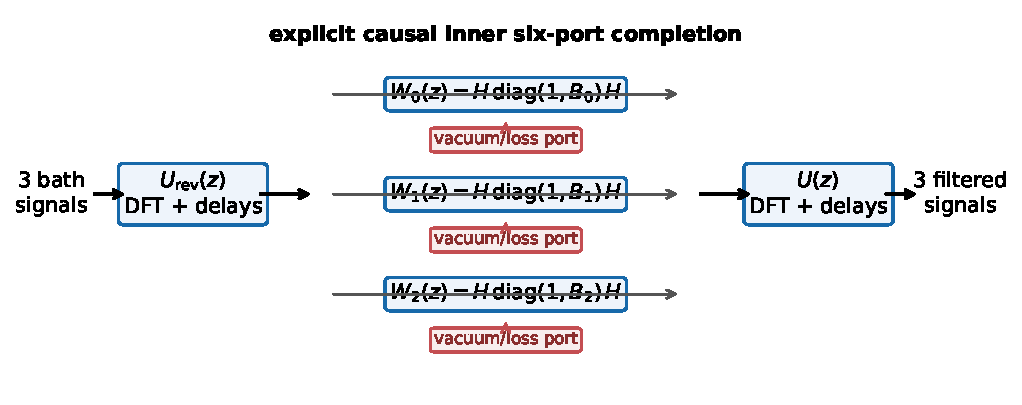
\includegraphics[width=0.94\linewidth]{figures/passive_architecture.pdf}
 \caption{Component-level realization.  The signal passes through a reverse
 paraunitary mixer, three parallel lossless Mach--Zehnder/all-pass blocks and a
 forward mixer.  The three auxiliary inputs are vacuum/loss ports.  Every
 displayed block is inner, so their cascade is inner.}
 \label{fig:architecture}
\end{figure}

\begin{proposition}[Physical passivity by construction]\label{prop:inner}
$\mathsf{S}_S$ is a causal rational inner six-port transfer and $G_S$ is a
rational Schur transfer in $\cR_S$.
\end{proposition}

\begin{proof}
$b_r$ is analytic in the unit disc and unimodular on $\T$.  Hence every
$B_g$, $W_g$, $W$, $U$, and $U_{\rm rev}$ is inner; products and block
diagonals preserve innerness.  The signal-block contraction follows from the
unitarity of the boundary completion.  The common denominator is
$(1-r_Sz)^S$.  The scalar $p_g$ numerators have degree at most $S$, while the
two mixers add at most four, so the numerator entries of $G_S$ have degree at
most $S+4$.
\end{proof}

The factorization is also a component prescription: three repeated scalar
all-pass elements, three balanced interferometers, a three-mode Fourier
network, and integer delays.  General passive-network realization results
\cite{GoughZhang2015,NurdinEtAl2016} provide a broader context, but are not
needed for the boundary unitarity identity used here.

\subsection{Pass nodes and full-spark signatures}

At a point where $B_g(z)=1$, let
\begin{equation}\label{eq:signature}
 v_{g,z}=U(z)e_g.
\end{equation}
Then $p_g(z)=1$ and the identity $U_{\rm rev}=z^2U^*$ gives
\begin{equation}\label{eq:exactcal}
 G_S(z)v_{g,z}=z^2v_{g,z}.
\end{equation}

\begin{lemma}[Node count]\label{lem:nodes}
For each $g\in\{0,1,2\}$, the open pass arc contains at least $S-1$ distinct
solutions of $B_g(z)=1$.
\end{lemma}

\begin{proof}
On the unit circle write $b_r(\e^{\mathrm{i}\theta})=
\e^{\mathrm{i}\beta_r(\theta)}$ with a continuous unwrapped phase on
$(-\pi,\pi)$ and
\[
 \beta_r'(\theta)=\frac{1-r^2}{1-2r\cos\theta+r^2}>0.
\]
For $r=r_S$, put $\beta_0=\beta_r(\pi/6)$.  The identity
\[
 \beta_0=2\arctan\!\left((2\e^{9S/20}-1)\tan\frac{\pi}{12}\right)
\]
and $\cot x<1/x$ show that $\beta_0>\pi(1-1/S)$ for every
$S\geq5$: the sufficient inequality
$(2\e^{9S/20}-1)\tan(\pi/12)>2S/\pi$ holds at $S=5$ and its
left-minus-right derivative is positive thereafter.  More directly, the inverse formula
\[
 \theta=2\arctan\!\left(\frac{1-r}{1+r}\tan\frac{\beta}{2}\right)
\]
maps the interval $(-\beta_0,\beta_0)$ into the pass arc.  The allowed interval
for the integer winding number in
$S\beta+\arg\eta_S+\phi_g=0\pmod{2\pi}$ has length
$S\beta_0/\pi>S-1$.  Every open real interval of length greater than $S-1$
contains at least $S-1$ integers, independently of the phase offset.  Hence at
least $S-1$ roots are interior.
\end{proof}

Select any $S-1$ nodes from each group and call the resulting set $\mathcal Z_S$;
its size is $M=3(S-1)$.  These signatures have a stronger property than
spanning collectively.

\begin{lemma}[Full spark]\label{lem:fullspark}
Every three distinct signatures in $\{v_{g,z}:(g,z)\in\mathcal Z_S\}$ are
linearly independent.
\end{lemma}

\begin{proof}
Multiplication by $F^*$ does not change independence, and
\[
 F^*v_{g,z}=3^{-1/2}(1,t,t^2)^\top,
 \qquad t=\omega^{-g}z.
\]
The three pass-node groups are rotated by $0,-2\pi/3,-4\pi/3$; their arcs are
disjoint, so distinct signatures give distinct $t$.  The determinant of any
three columns is the nonzero Vandermonde product
$3^{-3/2}(t_2-t_1)(t_3-t_1)(t_3-t_2)$.
\end{proof}

\subsection{Stopband leakage}

\begin{lemma}[Analytic stop envelope]\label{lem:stop}
On $\cI_{\rm s}$,
\begin{equation}\label{eq:eps}
 \|G_S(\e^{\mathrm{i}\theta})\|_{\op}
 \leq\varepsilon_S:=
 \left(\frac{\pi S}{6}+\frac12\right)\e^{-9S/20}.
\end{equation}
\end{lemma}

\begin{proof}
The mixers are unitary on $\T$, so the norm is $\max_g|p_g|$.  The all-pass
phase derivative is $S$ times the Poisson kernel.  On either stop arc,
$\cos\theta\leq-\sqrt3/2$, whence
\[
 \frac{1-r^2}{1-2r\cos\theta+r^2}\leq1-r^2.
\]
Starting from $B_S(-1)=-1$, its phase deviates from $\pi$ by at most
$S(1-r^2)\pi/6$.  Including $|\phi_g|\leq1-r$ and using
$|(1+\e^{\mathrm{i}(\pi+x)})/2|\leq|x|/2$ gives
\[
 |p_g|\leq\frac{\pi S}{12}(1-r^2)+\frac12(1-r)
 \leq\left(\frac{\pi S}{6}+\frac12\right)(1-r).
\]
Substitute $1-r=\e^{-\alpha S}$.
\end{proof}

\section{The architecture-separation theorem}

We can now state the central result.

\begin{theorem}[Passive irreducible/reducing separation]\label{thm:separation}
Fix $S\geq5$ and $\alpha=9/20$.  There are $M=3(S-1)$ pass nodes in
$\cI_{\rm p}$ and full-spark signatures such that:
\begin{enumerate}
 \item the signal block $G_S\in\cR_S$ has the explicit six-port inner
 completion \eqref{eq:sixport}, obeys all calibrations
 \eqref{eq:calibration}, and has stop leakage at most $\varepsilon_S$;
 \item every reducing $Q\in\cR_S$ obeying the same calibrations satisfies
 \begin{equation}\label{eq:comparatorlb}
   \|Q(z)\|_{\op}\geq1\qquad(z\in\cI_{\rm s});
 \end{equation}
 \item if such a comparator is Schur, equality holds in
 \eqref{eq:comparatorlb} throughout the stopband;
 \item whenever $\varepsilon_S<1$, $G_S$ is irreducible.
\end{enumerate}
Thus the signal-level architecture ratio is at least $1/\varepsilon_S$ and is
exponential up to the displayed polynomial prefactor.
\end{theorem}

\begin{proof}
The constructive statements follow from
\cref{prop:inner,lem:nodes,lem:fullspark,lem:stop}.  It remains to prove the
comparator obstruction.  Let $\C u$ be a reducing line of $Q$ and let $q$ be
its scalar branch.  Left-projecting each calibration with $u^*$ gives
\begin{equation}\label{eq:projected}
 (q(z_j)-z_j^2)\langle u,v_j\rangle=0.
\end{equation}
Full spark implies that at most two signatures lie in the plane $u^\perp$;
otherwise three would be dependent.  Consequently, $q-z^2$ vanishes at at
least
\[
 M-2=3S-5
\]
distinct boundary points.  After placing $q$ over the common denominator
$d$, the numerator of $q-z^2$ has degree at most $S+4$.  Since
$3S-5>S+4$ for $S\geq5$, the numerator is identically zero.  Therefore
$q(z)=z^2$ wherever regular, and
$\|Q(z)\|_{\op}\geq\|Q(z)u\|=1$.  A Schur comparator supplies the reverse
inequality.  Finally, if $G_S$ were reducing, the same result would force its
stop norm to be at least one, contradicting $\varepsilon_S<1$.
\end{proof}

\begin{remark}[What is held fixed]
Both sides have three signal channels, identical delayed directional
calibrations and the same rational bidegree ceiling.  The irreducible side is
also required to possess an explicit passive completion.  The lower bound is
proved for a larger comparison class that need not be passive; imposing
passivity only turns its lower bound into equality.
\end{remark}

\subsection{Approximate calibration and approximate reduction}

The exact obstruction has a quantitative counterpart.  Put $N=S+4$ and
$K=M-2=3S-5$, and define the full-spark singular margin
\begin{equation}\label{eq:gamma}
 \gamma_S=\min_{|J|=3}\sigma_{\min}[v_j]_{j\in J}>0.
\end{equation}
For an erasure set $E\subset\{1,\ldots,M\}$ of size two, let
$V_E=(z_j^k)_{j\notin E,\,0\leq k\leq N}$ and set
\begin{equation}\label{eq:chi}
 \chi_S=\min_{|E|=2}\sigma_{\min}(V_E)>0.
\end{equation}
Every $V_E$ has full column rank because it contains at least $N+1$ distinct
Vandermonde rows.  Finally take $R=8(S+1)$ fixed midpoint samples $\xi_\ell$
split equally across the two stop arcs, form
$W_S=(\xi_\ell^k)_{1\leq\ell\leq R,\,0\leq k\leq S}$, and put
\begin{equation}\label{eq:nu}
 \nu_S=\frac{\sigma_{\min}(W_S)}{\sqrt{R(S+1)}}>0.
\end{equation}

For $Q\in\cR_S$ and a unit vector $u$, define the calibration and sampled
left-reduction defects
\begin{equation}\label{eq:defects}
 \Delta(Q)=\max_j\|Q(z_j)v_j-z_j^2v_j\|,
 \quad
 \beta_u(Q)=\max_j\|(I-uu^*)Q(z_j)^*u\|.
\end{equation}
The second quantity vanishes for the reducing line used in
\cref{thm:separation}; allowing it to be small also covers approximate
one-way decoupling at the measured nodes.

\begin{theorem}[Quantitative approximate obstruction]\label{thm:robust}
For every $Q\in\cR_S$ and every unit $u$,
\begin{equation}\label{eq:robustlb}
 \sup_{\theta\in\cI_{\rm s}}\|Q(\e^{\mathrm{i}\theta})\|_{\op}
 \geq
 \left[1-C_S\bigl(\Delta(Q)+\beta_u(Q)\bigr)\right]_+,
 \qquad
 C_S=\frac{\sqrt{3K(N+1)}}{\gamma_S\chi_S\nu_S},
\end{equation}
where $[x]_+=\max\{x,0\}$.  In particular, this is a finite-error theorem
for every exactly reducing comparator by taking $\beta_u(Q)=0$.
\end{theorem}

\begin{proof}
Let $q=u^*Qu$.  Order the overlaps $|\langle u,v_j\rangle|$ and erase the
two smallest.  Applied to the triple of three smallest overlaps,
\eqref{eq:gamma} implies that the third, and hence every retained overlap, is
at least $\gamma_S/\sqrt3$.  Writing
$Q^*u=\overline q\,u+w$ at a calibration node gives
\[
 |(q(z_j)-z_j^2)\langle u,v_j\rangle|
 \leq\Delta(Q)+\beta_u(Q).
\]
Normalize the common denominator so that $\sup_\T|d|=1$, write $q=a/d$ and
$h=a-z^2d$.  Then $\deg h\leq N$ and, on the $K$ retained nodes,
\[
 |h(z_j)|\leq\sqrt3\,[\Delta(Q)+\beta_u(Q)]/\gamma_S.
\]
The least-squares bound from \eqref{eq:chi} gives
$\|c_h\|_2\leq\sqrt{3K}[\Delta(Q)+\beta_u(Q)]/(\gamma_S\chi_S)$, so
$\sup_\T|h|\leq\sqrt{N+1}\|c_h\|_2$.

It remains to prevent the denominator from hiding this estimate.  If $c_d$
is its padded coefficient vector, then
$1=\sup_\T|d|\leq\sqrt{S+1}\|c_d\|_2$.  Hence \eqref{eq:nu} guarantees a
fixed stop sample $\xi_\ell$ with $|d(\xi_\ell)|\geq\nu_S$.  At that point,
$|q-\xi_\ell^2|=|h/d|\leq C_S[\Delta(Q)+\beta_u(Q)]$, and therefore
$\|Q(\xi_\ell)\|_{\op}\geq|u^*Q(\xi_\ell)u|
\geq1-C_S[\Delta(Q)+\beta_u(Q)]$.
Taking the positive part proves the claim.
\end{proof}

The price of a denominator-free statement is visible in $C_S$.  More
importantly, the deterioration cannot be removed by a sharper proof.

\begin{theorem}[No uniform robustness for these calibrations]\label{thm:robustbarrier}
Let $C_S'$ be any constant for which
$\sup_{\cI_{\rm s}}\|Q\|_{\op}\geq[1-C_S'\Delta(Q)]_+$ holds for all reducing
Schur transfers in $\cR_S$.  Then
\begin{equation}\label{eq:necessaryC}
 C_S'\geq
 \frac{[1-\varepsilon_S]_+}{\sin(\e^{-9S/20}/2)}
 =2\e^{9S/20}(1+o(1)).
\end{equation}
\end{theorem}

\begin{proof}
Take the scalar transfer
$Q_{\rm c}(z)=z^2(1+B_S(z))I_3/2$.  It is Schur, reducing and belongs to
$\cR_S$.  At a calibration from group $g$, one has
$B_S(z_j)=\e^{-\mathrm{i}\phi_g}$, so its maximum calibration defect is
exactly $\sin(\e^{-9S/20}/2)$.  The central branch is one of the three scalar
arms in the construction, and \cref{lem:stop} gives
$\sup_{\cI_{\rm s}}\|Q_{\rm c}\|\leq\varepsilon_S$.  Substitution in the
assumed inequality yields \eqref{eq:necessaryC}; the asymptotic follows from
$\varepsilon_S\to0$ and $\sin x\sim x$.
\end{proof}

Together, \cref{thm:robust,thm:robustbarrier} replace a qualitative fragility
caveat by a precise statement: finite errors are controlled at every fixed
$S$, but the present increasingly clustered calibration family cannot support
an $S$-uniform tolerance theorem.

\section{Transfer to bath spectra and decoherence rates}

Let $J(\omega)$ be the $3\times3$ bath spectral-density matrix in a protected
frequency band.  Assume the uniform nondegeneracy condition
\begin{equation}\label{eq:bathbounds}
 j_-I\preceq J(\omega)\preceq j_+I,
 \qquad 0<j_-\leq j_+<\infty.
\end{equation}
For a linear passive prefilter $T$, the output noise spectrum is
\begin{equation}\label{eq:koss}
 \Gamma_T(\omega)=T(\e^{\mathrm{i}\theta(\omega)})
 J(\omega)T(\e^{\mathrm{i}\theta(\omega)})^*.
\end{equation}
In a weak-coupling Davies construction, $\Gamma_T$ is the Kossakowski matrix
sampled at the relevant Bohr frequency \cite{Davies1974}; in stationary
Gaussian pure dephasing it is directly the quadratic rate matrix.  The
following statement is linear algebra and therefore does not depend on a
particular master-equation normalization.

\begin{corollary}[Squared Kossakowski gap]\label{cor:rates}
On the stopband, the constructed signal block obeys
\begin{equation}\label{eq:rateupper}
 \|\Gamma_{G_S}(\omega)\|_{\op}
 \leq j_+\varepsilon_S^2.
\end{equation}
For every reducing calibrated comparator $Q\in\cR_S$, there is a fixed unit
direction $u$ such that
\begin{equation}\label{eq:ratelower}
 u^*\Gamma_Q(\omega)u\geq j_-
\end{equation}
throughout the stopband.  Hence the worst retained directional rate divided
by the constructed worst-case rate is at least
$j_-/(j_+\varepsilon_S^2)$.
\end{corollary}

\begin{proof}
Equation \eqref{eq:rateupper} follows from
$\|TJT^*\|\leq\|T\|^2\|J\|$.  For the comparator, the proof of
\cref{thm:separation} gives $Q^*u=\bar z^2u$ on $\T$.  Thus
\[
 u^*QJQ^*u=(Q^*u)^*J(Q^*u)\geq j_-\|Q^*u\|^2=j_-.
\]
\end{proof}

For a transition whose three coupling matrix elements form a vector $c$, its
Davies or pure-dephasing quadratic susceptibility is proportional to
$c^*\Gamma_Tc$.  Consequently \cref{cor:rates} gives an exact rate separation
for any model in which the relevant transition can probe the retained
direction $u$.  It also gives an architecture-independent upper bound for all
unit coupling vectors under $G_S$.

In pointer-basis pure dephasing, the coherence lifetime is inversely
proportional to the corresponding quadratic rate.  The construction therefore
permits a lifetime gain of order $\varepsilon_S^{-2}$ relative to the retained
comparator direction, subject to the Markov, stationarity and spectral-bounds
assumptions above.  Applying a maintenance inequality of the form
$P_{\rm extra}\geq k_BT\dot C_{\rm loss}$, as carefully delimited in
\cite{ErikssonCut2026}, transfers the rate comparison to the \emph{input of
the lower bound}.  A smaller lower bound does not prove an achievable low-power
maintenance protocol, and we do not use it that way.

\subsection{A closed Ramsey model with the vacuum ports included}

The signal-only congruence \eqref{eq:koss} does not by itself specify the
fluctuations entering the auxiliary ports.  Here is a minimal model in which
they are included rather than appended as an unknown correction.  Write the
signal output row of the full six-port inner transfer as $[T\ L]$ and take the
six-input symmetrized white-noise covariance to be
\begin{equation}\label{eq:closedinput}
 V_{\rm in}=\frac12 I_6+\begin{pmatrix}J&0\\0&0\end{pmatrix}.
\end{equation}
Thus every port contains vacuum, while the first three carry the additional
stationary Gaussian bath spectrum $J$.  Couple a pointer contrast $c\in\C^3$
linearly to the three output quadratures in the Markov pure-dephasing limit,
and absorb the convention-dependent coupling prefactor into the rate units.

\begin{proposition}[Vacuum-complete Ramsey rate]\label{prop:vacuumclosed}
For every passive six-port completion,
\begin{equation}\label{eq:closedcov}
 V_{{\rm out},{\rm sig}}=\frac12 I_3+TJT^*,
 \qquad
 \kappa_T(c)=\kappa_0\|c\|^2+c^*TJT^*c,
\end{equation}
where $\kappa_0$ is the common vacuum Ramsey rate in the chosen normalization.
Consequently the constructed network and every reducing calibrated comparator
$Q\in\cR_S$ that admits such a passive completion obey
\begin{equation}\label{eq:totalrates}
 \sup_{\|c\|=1}\kappa_{G_S}(c)
 \leq\kappa_0+j_+\varepsilon_S^2,
 \qquad
 \kappa_Q(u)\geq\kappa_0+j_-,
\end{equation}
and their certified total-rate advantage is at least
\begin{equation}\label{eq:vacuumratio}
 \frac{\kappa_0+j_-}{\kappa_0+j_+\varepsilon_S^2}.
\end{equation}
\end{proposition}

\begin{proof}
Unitarity of the signal output row gives $TT^*+LL^*=I_3$.  Applying
$[T\ L]$ on both sides of \eqref{eq:closedinput} therefore yields
\[
 \tfrac12(TT^*+LL^*)+TJT^*=\tfrac12I_3+TJT^*.
\]
Markov Gaussian pure dephasing turns the quadratic covariance in direction
$c$ into the Ramsey exponent, which gives \eqref{eq:closedcov}.  The two rate
bounds are then \cref{cor:rates} plus the same $\kappa_0$ term.
\end{proof}

This model makes two experimentally distinct claims.  Switching off the
excess bath preparation ($J=0$) measures $\kappa_0$ directly; switching it on
measures the excess rate $\kappa-\kappa_0$.  The latter retains the squared
exponential architecture gap, while the total lifetime benefit saturates at
$1+j_-/\kappa_0$ as $S\to\infty$ when $j_-=j_+$.  Vacuum therefore limits the
observable gain but does not invalidate or ambiguously renormalize it.  The
claim remains deliberately within a linear, Gaussian and Markov setting.

\section{The hidden resource: a delay-price theorem}

Exponential suppression in \cref{thm:separation} is obtained by taking
$r_S$ exponentially close to one.  This creates long-lived internal modes.
The next result shows that this is not an accident of our parameterization.

Let
\[
 B(z)=\xi\prod_{k=1}^S\frac{z-a_k}{1-\bar a_kz},
 \qquad |\xi|=1,\quad |a_k|<1,
\]
and $p=(1+B)/2$.  On the unit circle let $\tau_B(\theta)$ denote the unwrapped
phase derivative, or group delay in sample units:
\begin{equation}\label{eq:groupdelay}
 \tau_B(\theta)=\sum_{k=1}^S
 \frac{1-|a_k|^2}{|\e^{\mathrm{i}\theta}-a_k|^2}.
\end{equation}

\begin{theorem}[Stop suppression forces dwell time]\label{thm:delay}
Let $I\subset\T$ be a connected arc of angular length $L>0$.  If
$\sup_I|p|\leq\varepsilon<1$, then
\begin{equation}\label{eq:delaylb}
 \sup_{\theta\in[-\pi,\pi]}\tau_B(\theta)
 \geq \frac{LS}{16\arcsin\varepsilon}.
\end{equation}
\end{theorem}

\begin{proof}
The condition $|1+B|\leq2\varepsilon$ confines the phase of $B$ to an arc of
half-width $2\arcsin\varepsilon$ around $\pi$.  Because $I$ is connected and
$\varepsilon<1$, a continuous unwrapped phase cannot change branches inside
$I$; its total variation is at most $4\arcsin\varepsilon$.  On the other hand,
each Poisson kernel in \eqref{eq:groupdelay} obeys the uniform lower bound
\[
 \frac{1-|a_k|^2}{|\e^{\mathrm{i}\theta}-a_k|^2}
 \geq\frac{1-|a_k|}{4}.
\]
Integration over $I$ therefore yields
\[
 \frac{L}{4}\sum_{k=1}^S(1-|a_k|)
 \leq4\arcsin\varepsilon.
\]
For some $k_*$,
$1-|a_{k_*}|\leq16\arcsin(\varepsilon)/(LS)$.  At
$\theta=\arg a_{k_*}$, its Poisson kernel is
$(1+|a_{k_*}|)/(1-|a_{k_*}|)$, which alone is at least the right-hand side of
\eqref{eq:delaylb}.
\end{proof}

\begin{corollary}[Delay-budget frontier]\label{cor:delayfrontier}
Under the hypotheses of \cref{thm:delay}, let
$D=\sup_\theta\tau_B(\theta)$.  Then
\begin{equation}\label{eq:frontier}
 \varepsilon\geq\sin\!\left(\frac{LS}{16D}\right).
\end{equation}
Consequently, if $\delta=\varepsilon^2$ is the corresponding rate envelope,
the rate-improvement factor satisfies
\begin{equation}\label{eq:rate-delay}
 \frac1\delta\leq
 \csc^2\!\left(\frac{LS}{16D}\right)
 \sim\left(\frac{16D}{LS}\right)^2
 \qquad(D/S\to\infty).
\end{equation}
In particular, exponential rate improvement requires exponential peak delay
when $L$ is fixed and $S$ grows subexponentially relative to the target.
\end{corollary}

\begin{proof}
Rearrange \eqref{eq:delaylb} to obtain
$\arcsin\varepsilon\geq LS/(16D)$ and use monotonicity of sine on
$[0,\pi/2]$.  Squaring and inverting gives \eqref{eq:rate-delay}; the
asymptotic form follows from $\sin x\sim x$.
\end{proof}

For the repeated real zero in \eqref{eq:rdef}, the exact peak is
\begin{equation}\label{eq:ourdelay}
 \tau_{B_S}^{\max}=S\frac{1+r_S}{1-r_S}
 =S(2\e^{\alpha S}-1).
\end{equation}
Thus both the general lower bound and the construction are exponential when
the leakage is exponential, though the simple repeated-zero design is not
claimed constant-optimal.  In physical language, high-Q passive memory
replaces active pumping.  That is a real architectural benefit in settings
where storage time is cheap and drive power is expensive, but not a removal
of resource cost.  \Cref{cor:delayfrontier} makes the trade explicit: the
squared spectral-rate advantage can grow at most quadratically with available
peak delay, up to the order and arc-length factors shown.

\section{Numerical and exact verification}

The proofs above are analytic.  Computation audits implementation identities,
finite-precision behavior and scale.  The public replay performs:
\begin{enumerate}
 \item rational Gaussian elimination for \cref{prop:nogo};
 \item closed-form pass-node generation and all $\binom{M}{3}$ Vandermonde
 minor checks;
 \item dense global contractivity and stopband sweeps;
 \item direct $6\times6$ unitarity tests on 1001 boundary frequencies;
 \item the rational root-count inequality; and
 \item multiprecision evaluation of $\gamma_S,\chi_S,\nu_S$ and both sides of
 the robustness window; and
 \item the squared-rate, vacuum-covariance and group-delay identities.
\end{enumerate}
No optimizer is used to establish the theorem.

For the audit we fix $\alpha=0.45$.  \Cref{tab:audit} reports the observed
stop norm $\rho_S$, its square, the reciprocal rate factor, the exact peak
delay, and the maximum six-port unitarity residual.  The smallest full-spark
minor remains positive but becomes poorly conditioned by $S=19$; this is why
the numerical study stops there rather than presenting meaningless larger
orders.

\begin{table}[htbp]
\centering
\small
\setlength{\tabcolsep}{4.5pt}
\begin{tabular}{rrrrrr}
\toprule
$S$ & $M$ & $\rho_S$ & $\rho_S^2$ & $1/\rho_S^2$ & $\tau_{\max}$ \\
\midrule
5  & 15 & $1.269\,10^{-1}$ & $1.610\,10^{-2}$ & $6.21\,10^{1}$ & $8.99\,10^{1}$ \\
7  & 21 & $6.245\,10^{-2}$ & $3.900\,10^{-3}$ & $2.56\,10^{2}$ & $3.20\,10^{2}$ \\
9  & 27 & $2.990\,10^{-2}$ & $8.939\,10^{-4}$ & $1.12\,10^{3}$ & $1.02\,10^{3}$ \\
11 & 33 & $1.402\,10^{-2}$ & $1.965\,10^{-4}$ & $5.09\,10^{3}$ & $3.09\,10^{3}$ \\
15 & 45 & $2.940\,10^{-3}$ & $8.643\,10^{-6}$ & $1.16\,10^{5}$ & $2.56\,10^{4}$ \\
19 & 57 & $5.895\,10^{-4}$ & $3.475\,10^{-7}$ & $2.88\,10^{6}$ & $1.96\,10^{5}$ \\
\bottomrule
\end{tabular}
\caption{Dense-grid audit at $\alpha=0.45$.  All maximum calibration
residuals are below $6.3\times10^{-12}$ and all six-port unitarity errors below
$6.0\times10^{-14}$.  The theorem uses only $3(S-1)$ nodes; the replay audits
all $3S$ interior nodes found for these orders.}
\label{tab:audit}
\end{table}

\begin{figure}[htbp]
 \centering
 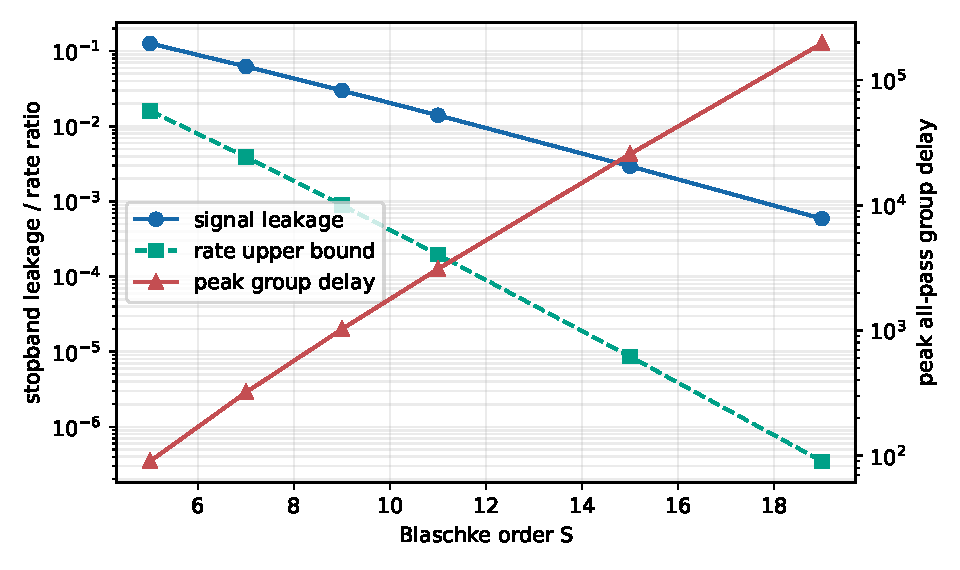
\includegraphics[width=0.82\linewidth]{figures/passive_scaling.pdf}
 \caption{Signal leakage and its squared rate envelope fall exponentially,
 while peak all-pass group delay rises exponentially.  Lines connect audited
 orders and are not statistical fits.}
 \label{fig:scaling}
\end{figure}

The observed rate factor exceeds $2.8\times10^6$ at $S=19$, but that number
should be read beside a peak delay near $2.0\times10^5$ samples and a minimum
Vandermonde minor near $1.3\times10^{-14}$.  The result is a theorem about
architecture and asymptotic possibility, not a claim that the largest audited
device is robustly fabricable.

\subsection{Passive-preserving tolerance stress test}

To distinguish algebraic existence from component tolerance, we run a frozen
Monte Carlo stress test at $S=11$.  Each of 2000 trials independently perturbs
the logarithm of each pole gap $1-r_g$ by a Gaussian standard deviation of
$1\%$, each arm phase by $1\%$ of the nominal pole gap, and each balanced
interferometer angle by $10^{-3}$ radians.  The seed is 20260810.  All
perturbations preserve $|B_g|=1$ and use orthogonal beam splitters, so every
trial remains a passive lossless six-port network; only its nominal calibration
is lost.

The median stop norm is $0.01421$, compared with the nominal $0.01402$; its
95th percentile is $0.01474$ and maximum is $0.01611$.  In contrast, the
maximum residual over the \emph{nominal} pass nodes has median $0.0700$ and
95th percentile $0.1293$.  Thus stop suppression is locally stable in this
component model, while exact high-order calibration is sensitive to pole
placement.  Retuning the pass frequencies restores exact roots for each
lossless sample, but a fixed-frequency application must budget this error.
The stress test supports the resource/conditioning caveat; it is not evidence
for a robust comparator separation.

\begin{figure}[htbp]
 \centering
 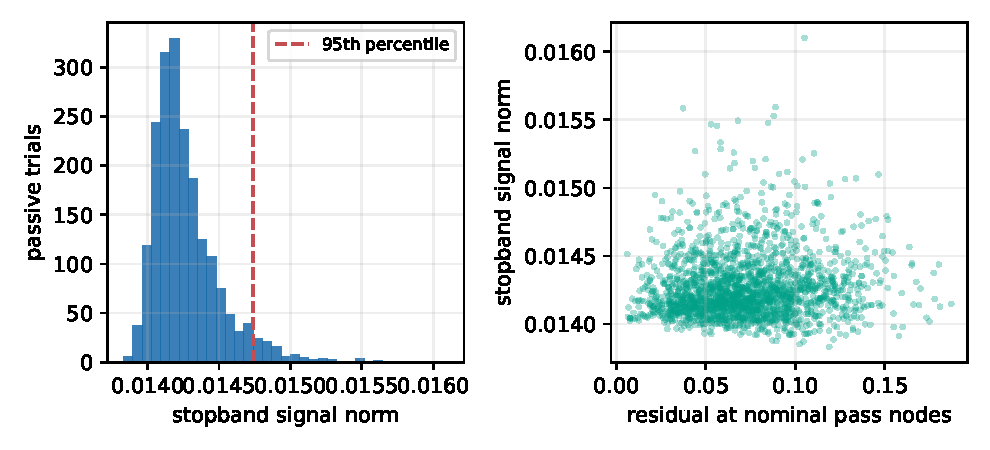
\includegraphics[width=0.84\linewidth]{figures/passive_tolerance.pdf}
 \caption{Passive-preserving tolerance audit at $S=11$ (2000 frozen trials).
 Stop leakage changes mildly, whereas residuals at the nominal calibration
 nodes expose the high-Q phase sensitivity.}
 \label{fig:tolerance}
\end{figure}

\subsection{Multiprecision robustness certificate}

Theorem~\ref{thm:robust} is analytic; its constants are finite because the
three displayed matrices have full column rank.  Nevertheless their scale is
scientifically relevant.  \Cref{tab:robust} evaluates them with 60 decimal
digits and reports both the proved $C_S$ and the necessary lower bound from
\cref{thm:robustbarrier}.  The enormous gap shows that our positive constant
is not sharp.  The rapid growth on both sides shows, without relying on Monte
Carlo perturbations, that fixed absolute tolerance is the wrong asymptotic
regime for these clustered nodes.

\begin{table}[htbp]
\centering
\small
\setlength{\tabcolsep}{4.0pt}
\begin{tabular}{rrrrrr}
\toprule
$S$ & $\gamma_S$ & $\chi_S$ & $\nu_S$ & $\log_{10}C_S$ & necessary $\log_{10}C_S'$ \\
\midrule
5 & $1.257\,10^{-3}$ & $4.676\,10^{-16}$ & $3.948\,10^{-5}$ & $23.873$ & $1.105$ \\
7 & $8.558\,10^{-5}$ & $6.528\,10^{-21}$ & $6.431\,10^{-7}$ & $31.825$ & $1.584$ \\
9 & $7.875\,10^{-6}$ & $2.124\,10^{-28}$ & $1.058\,10^{-8}$ & $42.235$ & $2.019$ \\
\bottomrule
\end{tabular}
\caption{Multiprecision conditioning audit for the quantitative obstruction.
The upper constant is a rigorous formula evaluated numerically, not a claim of
optimality.  The last column is a theorem-level lower bound on every possible
constant in an inequality of the same form.}
\label{tab:robust}
\end{table}

\subsection{Observable rate gap above a vacuum floor}

The six-port covariance identity in \cref{prop:vacuumclosed} is audited on a
257-point full-circle grid for every order in \cref{tab:audit}; the maximum
operator-norm residual is $1.46\times10^{-14}$.
\Cref{fig:closed} plots \eqref{eq:vacuumratio} for $j_-=j_+=1$ using the
observed leakage.  With no baseline it reproduces the squared spectral gap;
for every nonzero baseline it visibly approaches the predicted ceiling.  For
example, at $S=9$ and $\kappa_0/j=10^{-3}$ the certified total-rate factor is
$528.5$, while the zero-baseline excess-rate factor is $1118.7$.

\begin{figure}[htbp]
 \centering
 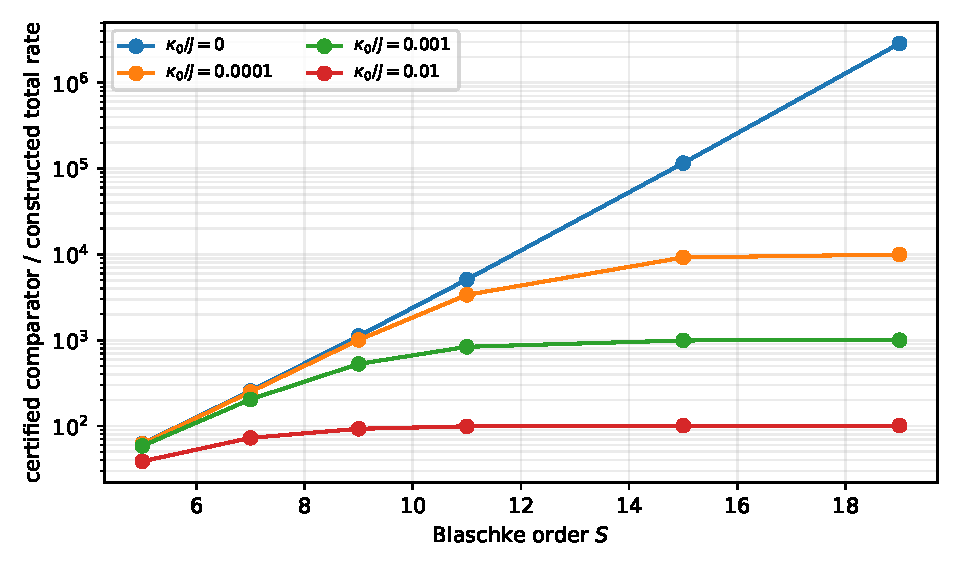
\includegraphics[width=0.82\linewidth]{figures/closed_dephasing.pdf}
 \caption{Certified total Ramsey-rate advantage after all vacuum inputs are
 included.  The auxiliary ports produce a common, independently measurable
 floor rather than an uncontrolled architecture-dependent correction.}
 \label{fig:closed}
\end{figure}

\section{Relation to prior work and novelty boundary}

Filter-function theory already supplies frequency-domain descriptions of
controlled open-system error \cite{PazSilvaViola2014,CerfontaineEtAl2021},
and experimental noise filtering is established \cite{SoareEtAl2014}.
Passive quantum feedback networks, lossless bounded-real transfers and
cascade realizations are likewise established
\cite{GoughJames2009,GoughGohmYanagisawa2009,GoughZhang2015,NurdinEtAl2016}.
Coherent passive reservoir engineering has, in particular, been formulated as
a pole-placement route to decoherence-free subsystems \cite{NguyenEtAl2018}.
Most directly, Techakesari and Nurdin preserve tangential responses and
passivity in model reduction \cite{TechakesariNurdin2017}; therefore neither
``tangential quantum interpolation'' nor ``physical interpolation'' is a
novelty claim here.  Tabak and Mabuchi connect Blaschke--Potapov factorization
to trapped modes in delayed passive quantum networks
\cite{TabakMabuchi2016}; therefore the use of Blaschke factors and the
interpretation of near-boundary poles as trapped memory are also prior art.

The new mathematical claim is the conjunction proved in
\cref{thm:separation,thm:robust,thm:robustbarrier,cor:rates,prop:vacuumclosed,thm:delay,cor:delayfrontier}: under one explicit collection of
full-spark delayed calibrations and one fixed rational bidegree, a passive
irreducible signal block has exponentially small stop leakage while every
constant-channel reducing transfer retains unit leakage; finite defects obey
an explicit conditioning bound that is provably nonuniform; a uniformly
nondegenerate bath squares the excess-noise gap and vacuum completion yields a
closed observable-rate formula; and strong scalar all-pass suppression forces
a quantitative peak-delay cost.  The earlier
matrix-polynomial paper \cite{ErikssonMIMO2026} supplied the classical
root-count architecture mechanism.  Here passivity, causal boundary phase,
an explicit quantum-compatible loss completion, the Kossakowski transfer and
the delay price change both the theorem and its interpretation.
Delay--bandwidth and storage--bandwidth tradeoffs are classical themes; the
paper claims neither theme in general.  The candidate novelty is the explicit
inequality used together with the fixed-bidegree architecture and bath-rate
separations.

\section{Limitations and falsification routes}\label{sec:limits}

\begin{limitation}[Conditioned rather than uniform robustness]
\Cref{thm:robust} propagates finite calibration and sampled reduction errors,
but its certified constants are extremely conservative.  Moreover,
\cref{thm:robustbarrier} proves that every theorem of this form deteriorates
at least exponentially for the present clustered calibration family.  A
fabrication-oriented successor should redesign the nodes and signatures or
optimize the finite interpolation constant; it cannot sharpen away the
nonuniformity established here.
\end{limitation}

\begin{limitation}[Linear stationary bath interface]
Equations \eqref{eq:koss} and \eqref{eq:closedcov} assume a linear filter and
a stationary Gaussian Markov bath.  General non-Gaussian or nonlinear
reservoirs need not transform by congruence, and strong-coupling or
non-Markovian dynamics need not be summarized by a Davies or Ramsey rate.
The vacuum ports are closed exactly inside the stated model, not outside it.
\end{limitation}

\begin{limitation}[No many-body mass-gap theorem]
The construction is a rational passive network, not an interacting quantum
field theory.  It neither proves a Yang--Mills mass gap nor establishes the
interacting-buffer conjecture in \cite{ErikssonCut2026}.  Its relevance is
methodological: it exhibits an exactly solvable architecture-dependent rate
boundary and the memory resource behind it.
\end{limitation}

\begin{limitation}[Restricted comparator]
The no-go covers the static reciprocal split of \cref{prop:staticsplit} at the
stated bidegree.  A device with higher rational degree, a dynamical
frequency-dependent change of channel coordinates, distinct input/output
splits, feedback outside the modeled ports or active gain lies outside the
theorem.  Those alternatives spend or change resources and remain possible
escape routes, not contradictions.
\end{limitation}

The most direct experimental falsification is a passive three-channel device
that satisfies the same calibrated responses and bidegree but has a verified
constant reducing line and stop norm below one.  Such a device would
contradict the algebraic root count and should be detectable from the public
calibration ledger.  A failure of the squared rate law under the stated
linear-Gaussian assumptions would instead falsify the bath-transfer model.

\section{Conclusion}

Irreducible channel mixing is not merely a coordinate choice when calibration
directions vary with frequency.  An explicit passive six-port family exploits
that fact to produce exponentially small signal leakage at a rational
complexity where every constant-channel reducing comparator retains a unit
branch.  The obstruction survives finite calibration and approximate
reduction errors with an explicit constant, while a scalar competitor proves
that uniform tolerance is impossible for the chosen nodes.  The bath spectral
density squares the separation in excess dissipative rates; a closed Ramsey
model turns every vacuum port into a measured common floor.  The same
construction exposes its own bill: exponentially long group delay, hence
high-Q passive memory.  Operationally, the Heisenberg cut can be displaced by
architecture, but the resource boundary reappears as dwell time, vacuum noise
and conditioning.  That simultaneous positive result, robustness barrier and
resource accounting is the central claim.

\section*{Code and data availability}

Source, exact-arithmetic checks, dense and multiprecision audits, the JSON
ledgers and the scripts that regenerate
\cref{fig:architecture,fig:scaling,fig:tolerance,fig:closed}
are available in the public
repository \cite{ErikssonRepository2026}:
\begin{center}
\href{https://github.com/lluiseriksson/finite-sample-spectral-certificates/tree/research/quantum-reservoir-boundary}{\texttt{Public source and verification branch}}
\end{center}
The principal commands are
\begin{verbatim}
python research/quantum_reservoir_filter.py
python research/quantum_reservoir_robustness.py
python research/quantum_reservoir_robust_bound.py
python research/quantum_reservoir_closed_dephasing.py
python verification/verify_passive_quantum_filter.py
\end{verbatim}
The release record pins the PDF and result-ledger hashes.  No private data,
remote service or stochastic seed is required.

\appendix
\section{A sharper view of the root-count obstruction}

Suppose a reducing comparator has a subspace of dimension two rather than a
declared reducing line.  Its orthogonal complement is a reducing line because
both the subspace and its complement are invariant by definition.  Therefore
the proof of \cref{thm:separation} loses at most two calibrations, regardless
of which nontrivial reducing dimension is initially supplied.

The degree $S+4$ is also conservative.  If the scalar branch numerator has
lower degree due to cancellation, the root-count contradiction becomes
stronger.  Boundary roots are legitimate because the denominator is assumed
regular on $\T$.  The proof does not require the comparator to be stable,
causal, passive or quantum realizable; those restrictions only shrink its
class.

\section{Bath congruence in a pure-dephasing model}

For completeness, consider coupling operators $A_a=A_a^*$ and bath fields
$B_a=B_a^*$ with interaction $H_I=\lambda\sum_{a=1}^3A_a\otimes B_a$.
At a fixed secular frequency, collect the bath correlations in
$J_{ab}(\omega)$.  A linear prefilter with annihilation-amplitude transfer $T$
maps the field vector to $T B$ (with the loss ports initially in vacuum), so
the signal contribution to its correlation matrix is $TJT^*$.  For a
transition $m\leftrightarrow n$, let
$c_a=\langle m|A_a|n\rangle$.  The associated quadratic dissipative
coefficient is, up to the common convention-dependent prefactor,
$c^*TJT^*c$.  This gives \eqref{eq:koss} for the excess-noise contribution.
For the closed white-noise model, collect the vacuum covariance of all six
inputs before adding $J$ on the signal ports.  The signal row identity
$TT^*+LL^*=I$ then gives \eqref{eq:closedcov}; no loss-port term remains
unspecified.  A colored or thermally populated auxiliary input would add its
known term $LJ_{\rm aux}L^*$ and would no longer be architecture independent.

For commuting pointer observables, the same calculation applies at zero Bohr
frequency to contrasts between pointer states.  If the contrast vector is
$c$, the off-diagonal density-matrix element decays as
$\exp[-\kappa(c)t]$ with $\kappa(c)$ proportional to
$c^*\Gamma_T(0)c$.  This is the exact pure-dephasing setting in which the
resource-boundary interpretation is cleanest.

\section{Reproducibility ledger}

The JSON record stores, for each $S$:
\begin{itemize}
 \item $r_S$, node count, numerator degree and root-count margin;
 \item minimum determinant magnitude over all signature triples;
 \item maximum calibration residual;
 \item global and stopband signal norms;
 \item the squared rate envelope and reciprocal factor;
 \item exact peak group delay; and
 \item maximum six-port unitarity residual.
\end{itemize}
Separate ledgers store the 60-digit singular margins and robustness constants,
and the closed-vacuum covariance residual and total-rate frontiers.
The analytic acceptance gates are deliberately looser than floating-point
roundoff: calibration residual below $10^{-9}$, unitarity residual below
$10^{-10}$, global norm below $1+2\times10^{-12}$, positive full-spark minors,
and stop norm below \eqref{eq:eps}.  A failed gate exits nonzero.

\bibliographystyle{unsrt}
\bibliography{references}

\end{document}
